\chapter{Analisi del problema}
\label{chap:analisi_problema}

\section{Obiettivo}
\label{sec:problema:obiettivo}
L'obiettivo di questa tesi è quello di studiare, progettare e realizzare un sistema autonomo in grado di eseguire una missione precedentemente impostata, utilizzando come sistema di navigazione la VO, nello scopo di analizzare dei marker noti e fissi. Il sistema è pensato per essere utilizzato in un ambiente chiuso, ad esempio un magazzino; di conseguenza, i marker dovrebbero essere posizionati sul soffitto, in modo tale da minimizzare la probabilità di non vederli; ma, per questioni di praticità, i marker vengono fissati al pavimento. \\
Gli obiettivi principali sono due:
\begin{itemize}
	\item Creare un sistema che cattura le immagini dalla camera, le analizza trovandone i marker e la loro posizione relativa all'ambiente e infine invia questi dati al flight controller.
	\item Sviluppare un programma che permetta di eseguire delle missioni precedentemente programmate e completamente personalizzabili. Le missioni saranno composte da una lista di obiettivi (target) e deve essere possibile impostare due modalità di target: la prima, in cui l'UAV arriva al punto scelto, si ferma fino a posizionarsi correttamente nel punto desiderato e poi continua la missione raggiungendo il punto successivo (hoverpoint); nella seconda modalità il drone arriva al target e passa direttamente al prossimo, senza fermarsi (waypoint).
\end{itemize}

\section{Soluzioni proposte in letteratura}
In letteratura sono presenti diverse strategie per risolvere il problema della localizzazione senza utilizzare la geolocalizzazione. Esse si dividono in due categorie: map-based e mapless \cite{CHANG2023104533}.
\begin{itemize}
	\item Map-based: a sua volta si dividono in due categorie: Known Map e Map-building.\\
	Nel primo caso, il sistema contiene delle informazioni sull'ambiente. Alcuni esempi sono la VO basata sui marker e l'utilizzo di radiofrequenze, dove attraverso l'analisi della Radio Signal Strength Indicator (RSSI) è possibile calcolare la distanza tra trasmettitore e ricevitore. In entrambi questi esempi è necessario che il drone sappia dove siano i marker/antenne per stimale la propria posizione. \\
	Nel secondo caso il sistema deve costruirsi internamente una mappa locale/globale dell'ambiente, mentre lo esplora. Questa tecnica viene chiamata Simultaneous Localization and Mapping (SLAM). Due esempi sono V-SLAM (sfrutta le immagini) e Lidar-SLAM (il lidar permette di calcolare il time-of-flight tra il sensore e l'ostacolo, di conseguenza la posizione).
	\item Mapless: esistono tre approcci: integrato, diretto e indiretto. nel primo approccio le informazioni dei sensori vengono direttamente trasformate in comandi per il drone, senza un'unità di controllo intermedia. L'approccio diretto estrae dalle immagini informazioni sull'ambiente e le invia a un'unità di controllo separata; quest'ultima ne determina i comandi di navigazione. Infine, l'approccio indiretto stima le distanze dagli ostacoli e fornisce queste informazioni a un'unità di controllo, che decide come modificare la traiettoria per evitare collisioni.
\end{itemize}
Per risolvere il nostro obiettivo la conoscenza della mappa è fondamentale, quindi le ricerce sono state concentrate in questa direzione.
\\ \\
A questo punto, i due approcci che possiamo confrontare sono Known Map e Map-building. Questo articolo \cite{7955787} confronta VO e SLAM, arrivando alla conclusione che la VO è l'approccio migliore perché risulta più veloce e richiede memoria e risorse computazionali inferiori rispetto a SLAM.
\\ \\
In questo articolo \cite{s22155798} propongono un UAV multirotore dove viene usata la VO basata sui marker come strumento di localizzazione. Il sistema proposto è pensato per la navigazione in ambienti al chiuso. Il sistema utilizza la seconda versione del Robot Operating System (ROS 2) \footnote{\url{https://www.ros.org/}} come libreria software per l'implementazione della VO; inoltre è stato scelto AprilTag come marker fiduciale. Un'altro articolo \cite{6549921} propone un sistema che sfrutta ROS per processare i dati arrivati dalla camera, mentre come marker propone l'utilizzo di ARTag. \\
In conclusione entrambi sistemi, anche se utilizzano architetture differenti, hanno dimostrato risultati più che sufficienti.
\\ \\
Un'altro approccio sempre basato sulla VO, ma senza l'utilizzo dei marker, è stato proposto in quest articolo \cite{4752770}. In molti edifici sono presenti dei soffitti con delle figure regolari, ad esempio un mosaico di quadrati. Il loro sistema consiste nel sfruttare queste figure per stimare posizione e posa del sistema, confrontando frame per frame l'immagine precedente con la successiva, e quindi stimando in che direzione il sistema si è spostato.
\\ \\
Tutte le architetture proposte in letteratura utilizzano il filtro di Kalman, un algoritmo matematico che restituisce un'ottima stima di posizione e posa del modello \cite{CHANG2023104533} \cite{7955787} \cite{8483685} \cite{s22155798} \cite{s19245480}. L'argomento viene approfondito nel paragrafo \ref{sec:problema:localizzazione:kalman}. 

\section{L’approccio proposto}
Analizzando gli obiettivi e i metodi proposti in letteratura, la soluzione proposta prevede l'utilizzo di un UAV dotato dei classici sistemi per il volo autonomo ad escluzione del ricevitore GPS, dato che non verrà utilizzato.  \\
Uno degli obiettivi è quello di creare un sistema che sfrutti la VO tramite marker per la localizzazione; di conseguenza è necessario installare sul drone con companion computer dotato di camera. È stato scelto un Raspberry Pi 3 con una camera OV7251 global shutter rivolta verso il basso, in modo tale che il sistema possa visualizzare il pavimento per poter localizzare i marker. Il Raspberry Pi 3, oltre ad eseguire il programma per la VO, deve ospitare il sistema per la gestione della missione. Entrambi i programmi sono scritti in Python, per questioni di praticità e sicurezza.\\
Tutte le comunicazioni tra il companion computer e il flight controller del drone vengono effettuate attraverso il protocollo MAVLink, sfruttando il GPIO (General Purpose Input/Output, una interfaccia hardware) del Raspberry e l'interfaccia seriale del flight controller Holybro Pixhawk 6C Mini. \\
Nelle sezioni \ref{sec:problema:localizzazione} e \ref{sec:problema:missione} vengono spiegate in modo più approfondito l'approccio adottato per la localizzazione e la missione.

\section{Sistema di localizzazione}
\label{sec:problema:localizzazione}
Come precedentemente spiegato, il sistema di localizzazione usa dei marker come punto di riferimento e, dopo l'elaborazione da parte del companion computer, i risultati saranno inviati al flight controller che li elaborerà per stimare posizione e posa. \\
In questo paragrafo vengono approfonditi questi due passaggi: la scelta del marker e come viene stimato lo stato interno dentro al flight controller.
\subsection{Marker}
In questo articolo \cite{fiducialMarker2021} viene svolta un'analisi di varie tipologie di marker usati nel campo della robotica. Quelli che vengono analizzati in modo più approfondito sono ARTag, AprilTag, ArUco e STag, ovvero quelli maggiormente utilizzati per l'obiettivo richiesto. \\ L'esperimento consiste nel testare ogni marker in condizioni di luce, posizione e orientamento, numero di marker visibili contemporaneamente e costo computazionale in base all'hardware scelto diversi. \\
Le conclusioni dell'esperimento mostrano che il marker ArUco presenta la miglior soluzione: ha presentato ottimi risultati nel calcolo della posizione e posa; un'ottima velocità di rilevamento; un buon costo computazionale e il migliore in termini di memoria utilizzata. D'altra parte, è molto sensibile in caso il marker sia molto piccolo oppure sia distante; infine il costo computazionale scala in base al numero di marker presenti dell'immagine. Il primo problema lo possiamo escludere dato che l'ambiente per cui il sistema è stato pensato è un posto chiuso, quindi la distanza massima del drone dal marker dipende dall'altezza dell'ambiente; il secondo problema non si può completamente risolvere, ma si può ridurre facendo un'analisi e scegliendo la posizione di ogni marker in base all'ambiente e alla missione che si dovrà eseguire, con l'obiettivo che la camera del drone visualizzi almeno un marker fino ad un massimo di quattro (perché vogliamo vederne almeno due, quindi nel caso peggione ne vediamo quattro). In Fig. \ref{fig:esempio_aruco} sono presenti un esempio di marker ArUco.
\begin{figure}
	\centering
	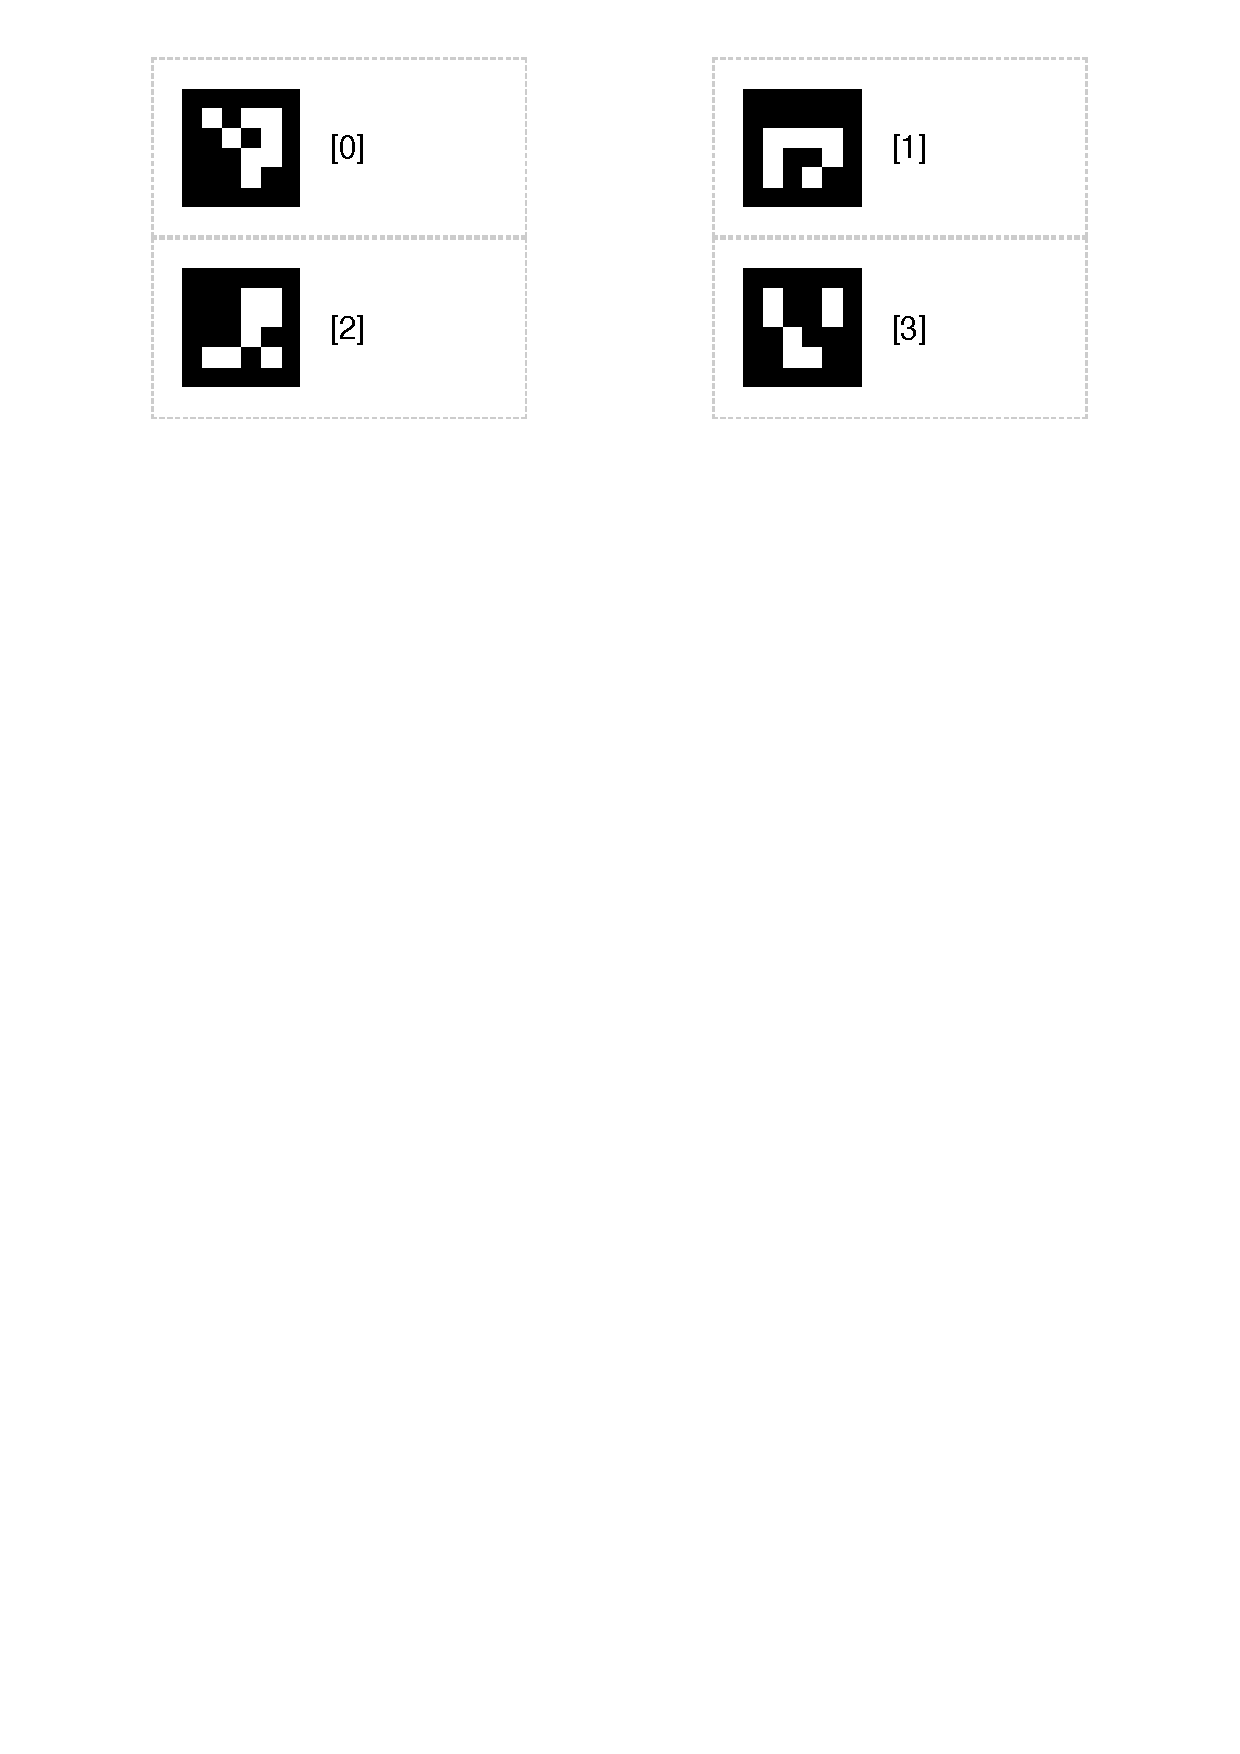
\includegraphics[width = 0.9\textwidth, trim={0 0 0 0}, clip]{immagini/esempio-aruco.pdf}
	\caption{Esempio di quattro marker ArUco 4x4 col il relativo ID.}
	\label{fig:esempio_aruco}
\end{figure}
\subsection{Filtro di Kalman}
\label{sec:problema:localizzazione:kalman}
Analizzando il sistema, possiamo pensare che solamente la VO ci dia le informazioni di posizione e posa dell'UAV; in realtà, dentro al flight controller esiste un'altro componente che direttamente o indirettamente può darci le stesse informazioni, ovvero l'IMU (Inertial Measurement Unit). Questo dispositivo contiene all'interno vari componenti: accellerometro, giroscopio e opzionalmente un magnetometro; a noi interessano i primi due: il primo ci permette di stimare la posizione del drone rispetto alle sue coordinate di partenza, sfruttando la lettura delle accellerazioni subite; mentre il secondo dispositivo ci fornisce le informazioni di posa. Tuttavia l'IMU ha un grosso problema, ovvero che l'errore di stima della posizione aumenta con il passare del tempo; questo è dovuto dal fatto che il sensore, anche se calibrato correttamente, presenta un'incertezza che si propaga nel tempo (drift); di conseguenza, quando viene calcolata la doppia integrazione per passare dall'accellerazione alla posizione, l'errore diventa esponenziale. \\
Questo non vuol dire che dobbiamo buttare le informazioni dell'IMU; possiamo fonderle ai dati che ci arrivano da altri sensori più affidabili, ad esempio dal GNSS o dalla VO. Questo è possibile attraverso un algoritmo matematico ricorsivo chiamato filtro di Kalman; esso permette di stimare lo stato interno di un sistema dinamico a partire da una sequenza di misurazioni che presentano rumore e incertezza. In particolare, nei droni viene usata una sua variante chiamata Extended Kalman Filter (EKF), che permette di gestire sistemi non lineari.
\\
\begin{figure}
	\centering
	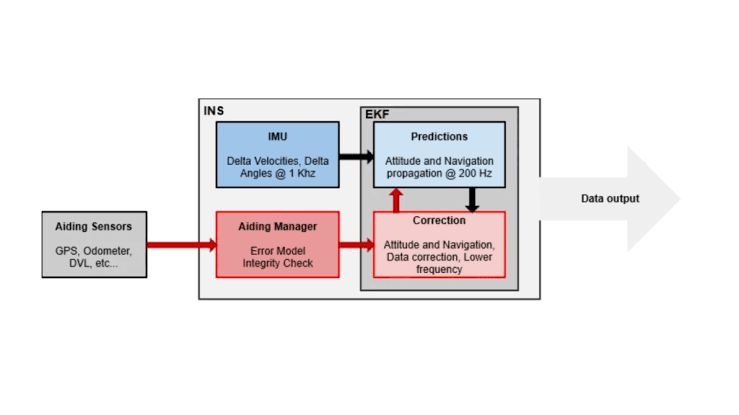
\includegraphics[width = 1\textwidth, trim={0 0 0 0}, clip]{immagini/filtro-kalman.png}
	\caption{Principio base del funzionamento di un Extended Kalman Filter (EKF).}
	\label{fig:esempio_ekf}
\end{figure}
\\
L'EKF utilizzato nel PX4 Autopilot è la versione due, chiamato EKF2\footnote{\url{https://docs.px4.io/main/en/advanced_config/tuning_the_ecl_ekf}} \footnote{\url{https://www.youtube.com/watch?v=CMGQJNPiTJg&t=39s}}.

\section{Struttura della missione}
\label{sec:problema:missione}
La missione viene descritta attraverso un file json e contiene una lista di target da raggiungere. Ogni obiettivo ha vari parametri, alcuni opzionali e alcuni no:
\begin{itemize}
	\item {\em north\_m, east\_m, down\_m} (obbligatori): indicano le coordinate NED della posizione dell'obiettivo che si vuole raggiungere, rispetto al sistema di riferimento locale. La posizione è espressa in metri.
	\item {\em yaw\_deg} (opzionale): esprime l'angolo yaw desiderato in gradi. Il valore di default è 0.
	\item {\em hover\_time\_ms} (opzionale): indica il tempo di attesa del drone, dopo aver correttamente raggiunto l'obiettivo corrente, prima di passare al prossimo obiettivo. Viene espresso in millisecondi. Il valore di default è 0.
	\item {\em vel\_m\_s} (opzionale): esprime la velocità che l'UAV avrà fino al raggiungimento del target o in prossimità di esso, espressa in metri al secondo. Il suo valore di default è null, e rappresenta l'assenza di impostare una velocità fissa.
	\item {\em expiration\_time\_s} (opzionale): indica il tempo dopo il quale il target in corso scade. La velocità del drone viene impostata in modo tale che l'UAV possa raggiungere il target nel tempo prestabilito. È espresso in secondi. Il suo valore di default è null, e rappresenta l'assenza del tempo di scadenza del target.
\end{itemize}
Le due modalità di target che sono fissate come obiettivi sono hoverpoint e waypoint. Un metodo per eseguire la prima modalità è senza impostare i valori {\em vel\_m\_s} o {\em expiration\_time\_s}; in questo modo, l'UAV prima di passare al prossimo obiettivo deve raggiungere correttamente quello corrente. Invece usando uno di questi parametri è possibile impostare il target in modalità waypoint.